\documentclass{liostyle}

\renewcommand{\taskname}{draugai} % in lowercase letters
\renewcommand{\longtaskname}{Draugai} % the title
\renewcommand{\version}{1.0}

%Constraints
\newcommand{\maxN}{1\ 000\ 000}

\begin{document}

\begin{wrapfigure}{r}{4cm}
\vspace{-20pt}
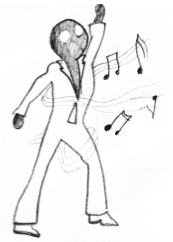
\includegraphics[width=3.8cm]{draugai_fig1}
\vspace{-20pt}
\end{wrapfigure}

Justas nori surengti vakarėlį ir planuoja pasikviesti kuo 
daugiau draugų. Tačiau jo draugai skirtingi: vieni mėgsta 
švęsti triukšmingai, didelėje kompanijoje, o kitiems labiau 
patinka švęsti ramioje, jaukioje aplinkoje, su keletu gerų 
draugų.

%\begin{figure}[h]
%\centering
%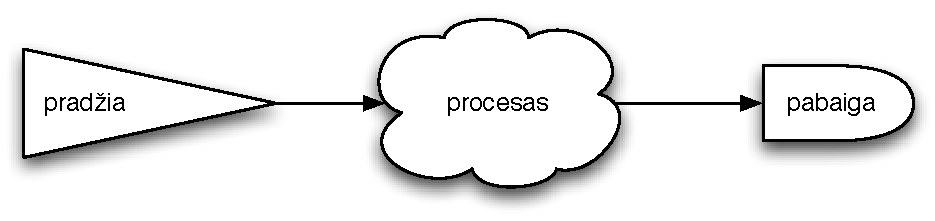
\includegraphics[width=0.8\textwidth]{draugai_fig2}
%\end{figure}

Justas atliko apklausą ir kiekvienas draugas jam pasakė, kiek 
mažiausiai ir kiek daugiausiai žmonių (įskaitant jį patį bei 
Justą) gali dalyvauti vakarėlyje, kad jis sutiktų atvykti. Jei
žmonių bus per daug arba per mažai – jis neatvyks.

\Task
Justas nori triukšmingo vakarėlio. Parašykite programą, kuri pasiūlytų 
Justui, kuriuos draugus jis turėtų kviestis, kad vakarėlyje dalyvautų kuo daugiau 
žmonių.

\Input
Pirmoje eilutėje įrašytas Justo draugų skaičius $\mathbf{N}$
($1 \le \mathbf{N} \le \maxN$). Kiekvienoje tolesnių eilučių yra po du skaičius
$m_i$ ir $d_i$ ($2\le m_i\le d_i\le \mathbf{N}+1$), nurodančius, kiek
mažiausiai ir kiek daugiausiai žmonių gali dalyvauti vakarėlyje, kad $i$-asis
draugas sutiktų prisijungti.

Laikoma, kad draugai sunumeruoti nuo 1 iki $\mathbf{N}$ ir informacija apie
juos pateikiama numerių didėjimo tvarka.

\Output
Pirmoje eilutėje įrašomas maksimalus pakviestų draugų skaičius $\mathbf{K}$.
Likusiose $\mathbf{K}$ eilučių~-- kviečiamų draugų numeriai. Jei galimi keli sprendiniai,
pateikite bet kurį.

\Examples
\example{
7
5 5
3 6
2 4
4 8
3 6
3 5
6 8
}{
4
1
2
4
5
}{
Daugiausia galima pakviesti keturis draugus,
pavyzdžiui 1-ą, 2-ą, 4-ą ir 5-ą. Iš
viso vakarėlyje dalyvaus penki asmenys (su
Justu).

1-asis draugas ateis, nes jis nori, kad
vakarėlyje dalyvautų lygiai 5 asmenys. 

2-asis draugas ateis, nes jis nori, kad
vakarėlyje dalyvautų nuo 3 iki 6 asmenų. 

4-asis ateis, nes jis nori, kad dalyvautų nuo
4 iki 8 asmenų;

5-asis ateis, nes jis nori, kad vakarėlyje
dalyvautų nuo 3 iki 6 asmenų.

Galimi ir kiti sprendiniai.
}

\Grading
Už testus, kuriuose $\mathbf{N} \le 10\ 000$, galima surinkti iki 50\% balų.

\Constraints
$1 \le \mathbf{N} \le \maxN$,\enskip
$2\le m_i\le d_i\le \mathbf{N}+1$.

\end{document}

